


\subsubsection{Tratamento dos dados}

\paragraph{Normalização} \par
\text{ }  \par

A normalização foi deixada para ser aprendida nos modelos, sendo que todos os modelos têm a normalização como segunda camada.\par

\paragraph{Limpeza} \par
\text{ }  \par

Podemos ver pelos gráficos seguintes que a existem alguns \textit{outliers}, sendo estes definidos como 3 (três) desvios padrão de distância à média.\par
Estes gráficos mostram também que existe uma variação do que são os valores normais de cada atributo a nível temporal. Logo um método de limpeza não se poderia basear apenas numa definição geral de \textit{outliers}, mas teria também de ser feito em janelas temporais.\par
Pelo mesmo argumento e visto que os \textit{outliers} fazem parte do que queremos também descobrir, não é aplicada nenhum método de remoção dos mesmo, sendo os dados passados a cru para os modelos.\par


\begin{figure}[H]
  \centering
  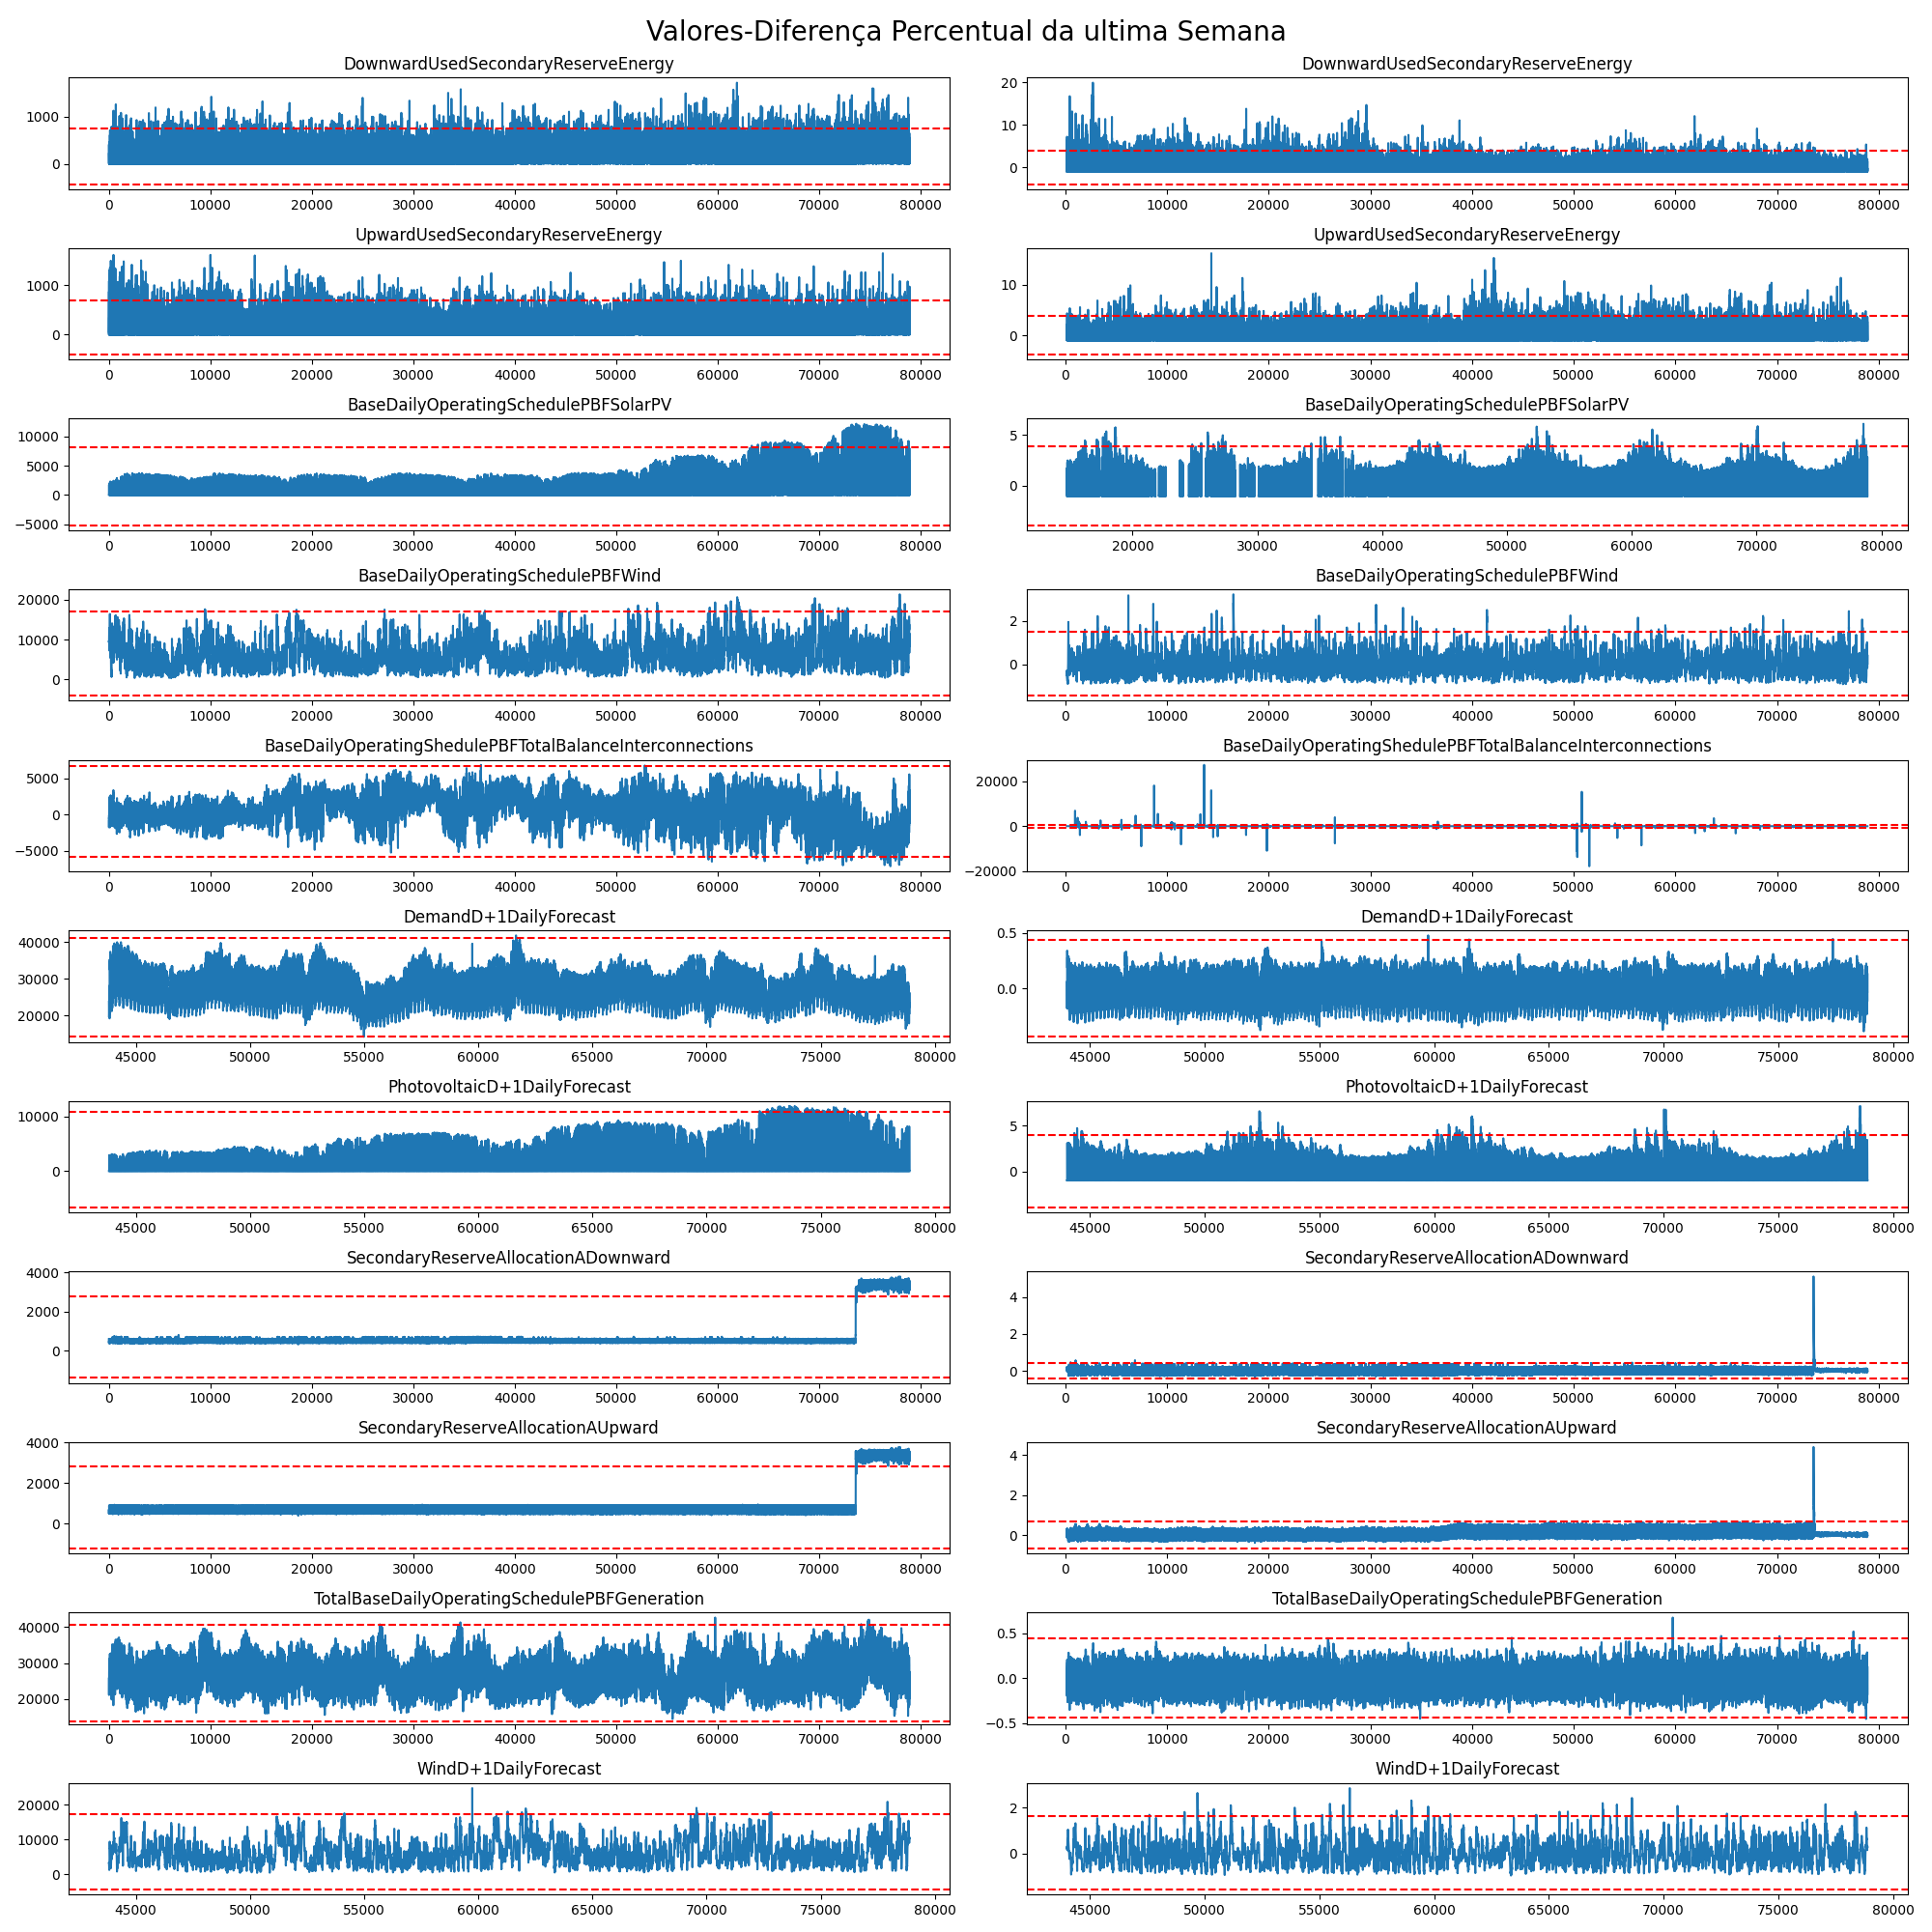
\includegraphics[width=\textwidth]{plots/Outliers_3stds.png}
  \caption{Outliers}
\end{figure}

Com outra análise desta variação dos atributos a nível temporal verificou-se que qualquer divisão dos dados para treino e teste deva levar as variações em consideração. Com efeito, o treino deve ter representatividade de todas as condições diferentes, ou pelo menos, da maior parte delas.\par


\paragraph{Dados em falta (\textit{Missing Data})}
\text{ }  \par

Estudemos também o caso de dados em falta. Alguns destes atributos têm certas entradas vazias, e como é possível verificar, alguns não têm determinados anos inteiros.\par
Como é nossa intenção usar o máximo de dados possíveis, usaremo nesses dados usar técnicas de \textit{imputing}.\par
Vendo no gráfico abaixo, verificamos que temos dados em falta de vários anos, em três atributos, e um deles tem algumas horas esporádicas em falta nos primeiros anos.\par

\begin{figure}[H]
  \centering
  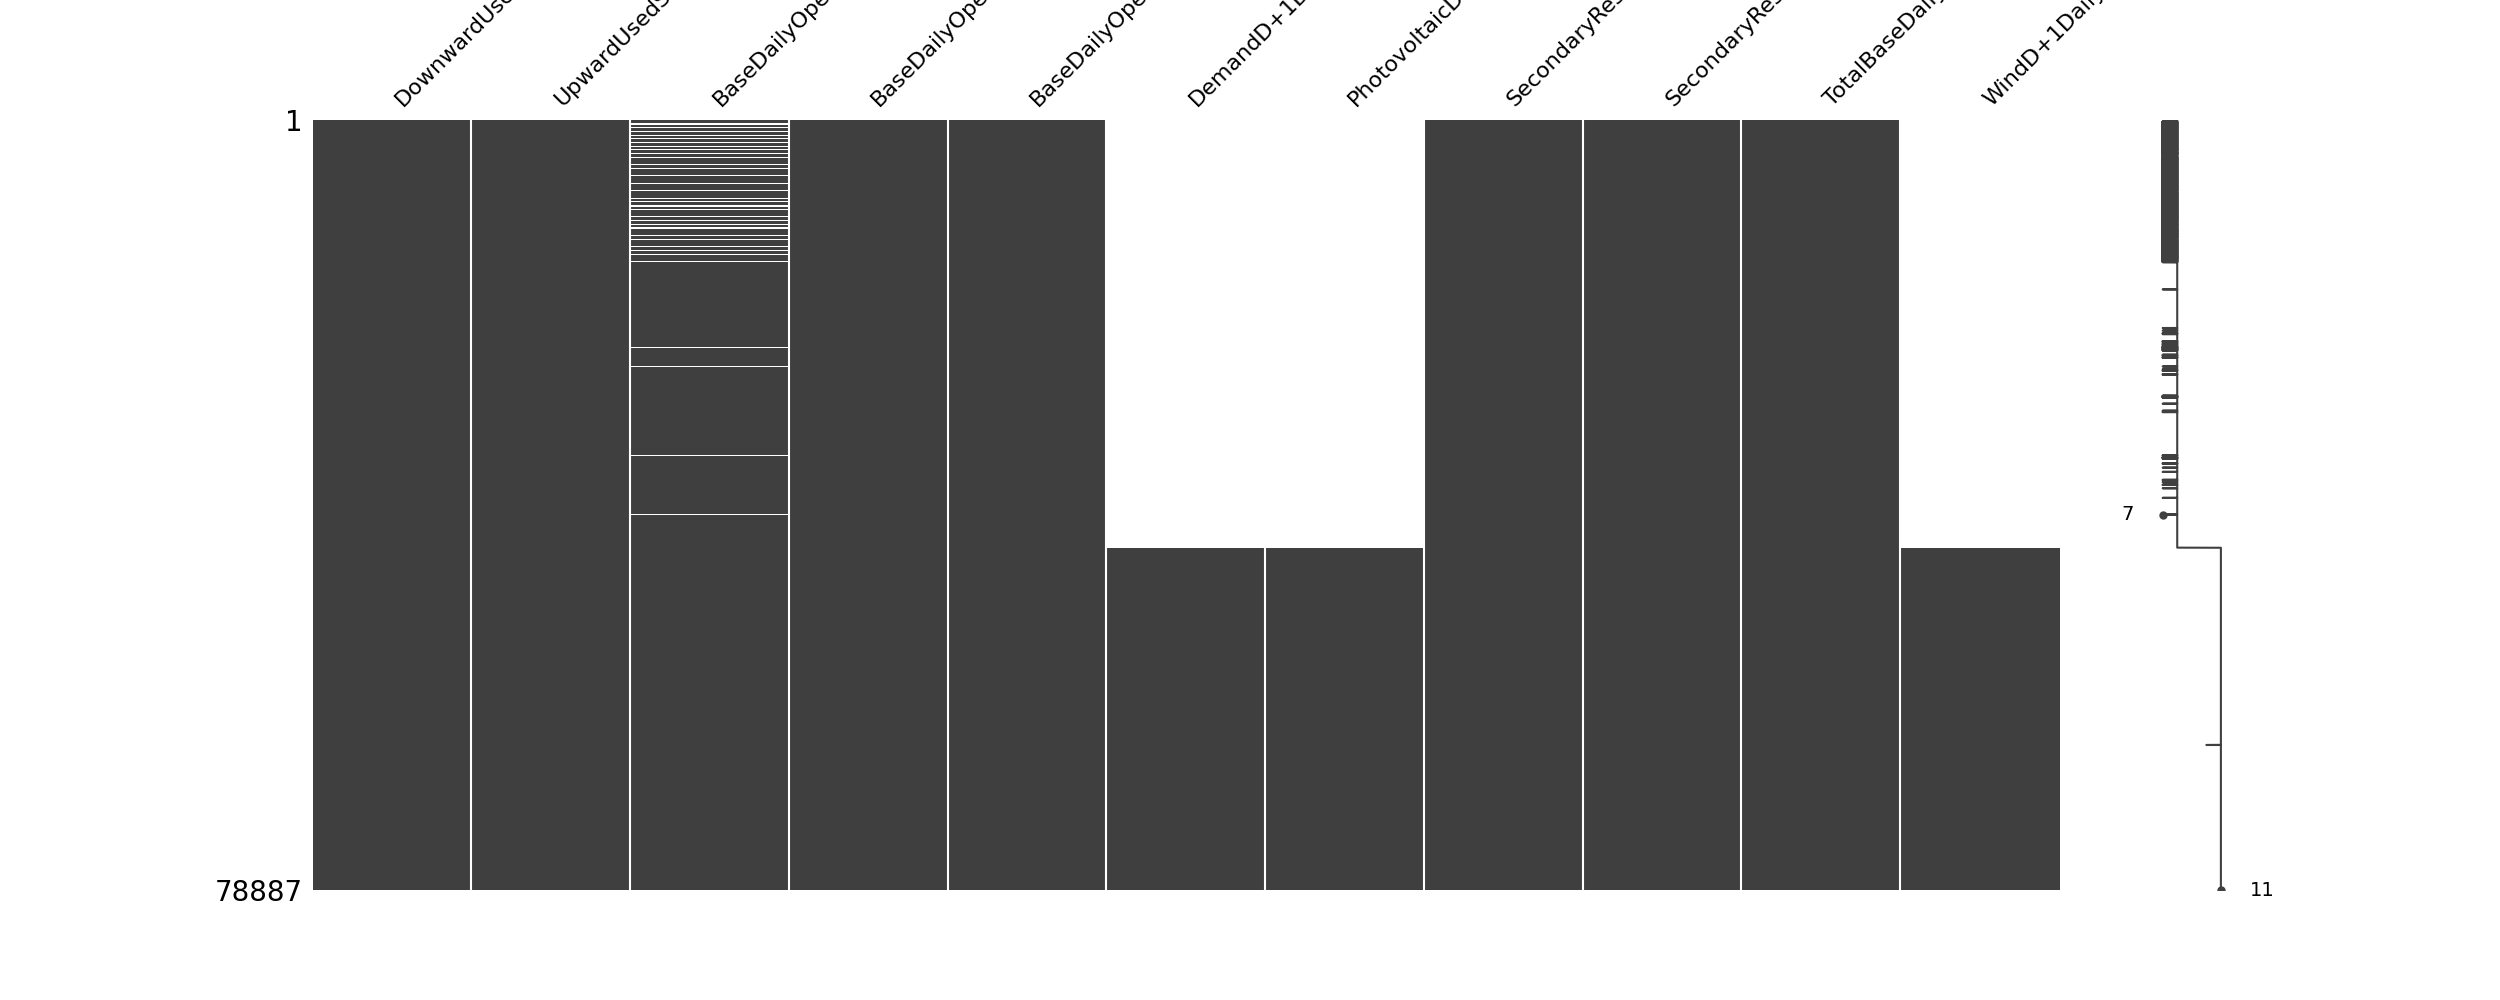
\includegraphics[width=\textwidth]{plots/missing_data.png}
  \caption{Dados em falta}
\end{figure}

Vamos aplicar o método experimental \href{https://scikit-learn.org/stable/modules/generated/sklearn.impute.IterativeImputer.html}{IterativeImputer} da biblioteca de \textit{python} \href{https://scikit-learn.org/stable/index.html}{sklearn}.\par
Este método é baseado nos trabalhos de \cite{vanBuuren2011} e de \cite{Buck1960}.\par
Por ultimo foi adicionado ao dados mais atributos, sendo eles todos de cariz temporal. São adicionados atributos correspondentes à hora, ao dia do ano, ao dia da semana, ao dia do mês, mês, ano.\par

